\chapter{Εισαγωγή}

\par
Το αντικείμενο της δημιουργίας περιεχομένου(Content Generation) είναι ένα πεδίο της Τεχνητής Νοημοσύνης με εφαρμογές στην ανάπτυξη ηλεκτρονικών παιχνιδιών, στην μουσική, στις ταινίες και σε πολλούς ακόμα τομείς. Μπορούμε να διακρίνουμε δύο διαφορετικές κατηγορίες δημιουργίας περιεχομένου με βάση τα είδη των αλγορίθμων που εφαρμόζονται σε κάθε κατηγορία. Αυτή η εργασία ερευνά τις δύο αυτές κατηγορίες και την αλληλεπίδραση που μπορεί να δημιουργηθεί μεταξύ τους.
\par
Η πρώτη κατηγορία αφορά τη δημιουργία περιεχομένου με τη χρήση κλασσικών αλγορίθμων (Procedural Content Generation), και η δεύτερη κατηγορία περιέχει την δημιουργία περιεχομένου με την χρήση μηχανικής μάθησης (Machine Learning based PCG). Η μέθοδος του Procedural Content Generation (PCG), είναι η παλαιότερη από τις δύο και αυτή με τις περισσότερες εφαρμογές και ερευνητικό περιεχόμενο. Η μέθοδος του Machine Learning (ML based PCG) έχει γνωρίσει μεγάλη ανάπτυξη τα τελευταία χρόνια και αποδίδει εντυπωσιακά αποτελέσματα όπου εφαρμόζεται με σωστή έρευνα και ανάπτυξη.

\section{Στόχοι της εργασίας}
\par
Ο βασικός στόχος αυτής της εργασίας είναι η μελέτη δύο διακριτών μεθόδων παραγωγής δισδιάστατων επιπέδων παιχνιδιού. Ως επίπεδο ορίζουμε τον χώρο  στον οποίο μπορεί να περιηγηθεί και να αλληλεπιδράσει ο παίκτης. Τα επίπεδα πρέπει να έχουν κάποια συγκεκριμένα χαρακτηριστικά, σε απλοποιημένη μορφή όπως δωμάτια, διάδρομοι και τοίχοι, σε μια λογική διάταξη.
\par
Η πρώτη από τις δύο μεθόδους αφορά ένα PCG σύστημα παραγωγής επιπέδων με τα συγκεκριμένα χαρακτηριστικά. Για την δημιουργία των επιπέδων χρησιμοποιούνται γνωστοί αλγόριθμοι PCG και τυχαίες τιμές για την διαφοροποίηση συγκεκριμένων χαρακτηριστικών ανάμεσα στα επίπεδα.
\par
Η δεύτερη μέθοδος αφορά ένα ML σύστημα, και συγκεκριμένα ένα Generative Adversarial Network (GAN). Το σύστημα αυτό θα λαμβάνει ως είσοδο εκπαίδευσης επίπεδα που δημιουργήθηκαν από το PCG σύστημα με σκοπό να παράγει επίπεδα αντίστοιχης ποιότητας μόλις του ζητηθεί.
\par
Αν και η αναπαράσταση των επιπέδων κρατήθηκε πολύ απλή, υπάρχουν πολλές δυσκολίες που πρέπει να επιλυθούν και για τις δύο μεθόδους ώστε να παραχθούν ικανοποιητικά αποτελέσματα.

\section{Προκλήσεις και δυσκολίες}
\par
Η μεγαλύτερη πρόκληση που αντιμετωπίστηκε κατά την ανάπτυξη αυτής της εργασίας, ήταν η σχεδίαση της αρχιτεκτονικής που θα έχει το μοντέλο του GAN στο ML σύστημα. Το GAN είναι ένα είδος νευρωνικού δικτύου, και η αρχιτεκτονική του αφορά το είδος, την ιεραρχία και τις παραμέτρους των επιπέδων που το αποτελούν. Η αρχιτεκτονική του νευρωνικού δικτύου αλλάζει σημαντικά ανάλογα με το είδος της εφαρμογής στην οποία θα εφαρμοστεί. Για τις εφαρμογές \textit{ανάπτυξης περιεχομένου} δεν υπάρχουν πολλές υλοποιήσεις διαθέσιμες, ειδικά με τα κριτήρια που απαιτούνται στο συγκεκριμένο πρόβλημα. Συνεπώς η αρχιτεκτονική του δικτύου βρέθηκε μετά από πολλές δοκιμές και πειραματισμούς.
\par
Όπως αναφέρθηκε, η κατηγορία της δημιουργία περιεχομένου με την χρήση μηχανικής μάθησης είναι πολύ πιο πρόσφατη και λιγότερο διαδεδομένη από την κατηγορία του PCG. Συνεπώς έχει λιγότερα παραδείγματα και βιβλιογραφία από την οποία μπορούμε να πάρουμε ιδέες και λύσεις. Αυτή η δυσκολία είναι που την κάνει και πιο ενδιαφέρουσα.
\par
Μια ακόμα δυσκολία που αντιμετωπίστηκε ήταν η μεταφορά των επιπέδων μεταξύ συστημάτων. Τα δύο συστήματα, PCG και ML, είναι ανεπτυγμένα σε διαφορετικές γλώσσες προγραμματισμού, έχουν διαφορετικά είδη δεδομένων και πρέπει να μπορούν να διαβάζουν και να αποθηκεύουν τα επίπεδα με μια κοινή μορφή. Αυτό είχε μια επιπλέον δυσκολία για το ML σύστημα καθώς τα δεδομένα πρέπει να περάσουν από ένα στάδιο προ-επεξεργασίας, το οποίο τα αλλοιώνει, συνεπώς πριν την αποθήκευση τους από το ML σύστημα έπρεπε να περάσουν από την αντίστοιχη προ επεξεργασία με την αντίθετη μετατροπή για να είναι αναγνώσιμα από το σύστημα PCG.

\begin{figure}[H]
\centering
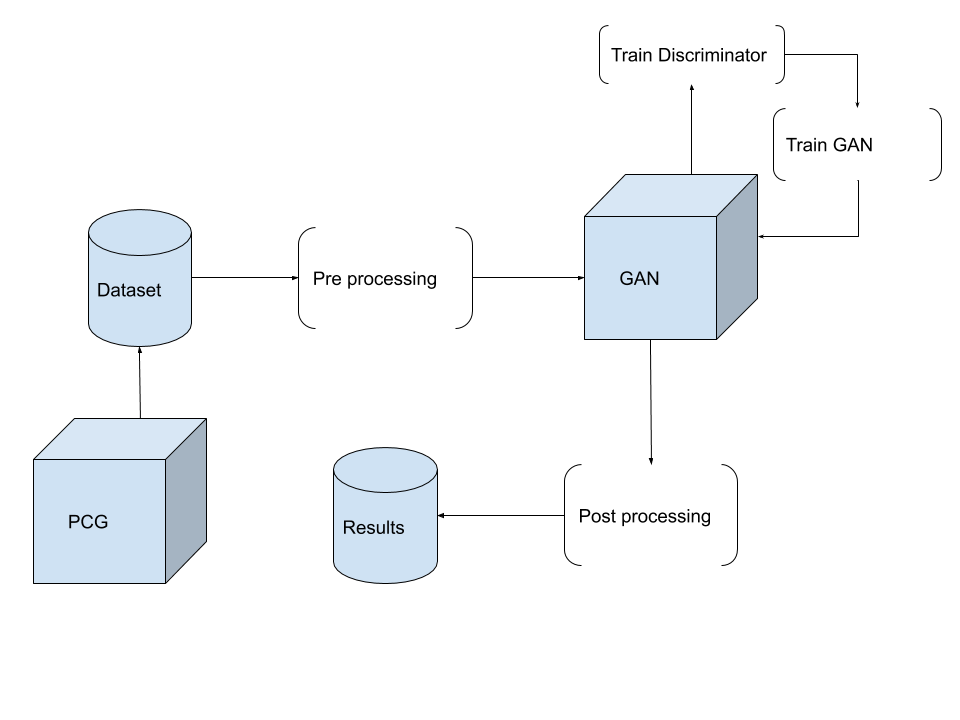
\includegraphics[width=.8\linewidth]{../images/graphs/Data_Cycle.png}
\caption{Σχεδιάγραμμα λειτουργίας των συστημάτων PCG και GAN}
\label{fig:fig}
\end{figure}




\section{Περιεχόμενα}
Στο κεφάλαιο 2 γίνεται μια περιγραφή της θεωρίας και εννοιολογίας του PCG καθώς και μερικών αντιπροσωπευτικών αλγορίθμων. Στο κεφάλαιο 3 αναλύεται πως υλοποιήθηκε το σύστημα PCG σε αυτή την εργασία, σε αναφορά και με το προηγούμενο κεφάλαιο. Με την ίδια λογική, στο κεφάλαιο 4 γίνεται μια θεωρητική ανάλυση του τομέα του ML, με έμφαση στις μεθόδους που χρησιμοποιήθηκαν στην υλοποίηση η οποία αναλύεται στο κεφάλαιο 5 μαζί με τα αποτελέσματα που παρήχθησαν από την εκπαίδευση του συστήματος ML. Στο προτελευταίο κεφάλαιο, 6, αναλύουμε τα συμπεράσματα που προέκυψαν από αυτή την εργασία και μελλοντικές προτάσεις. Το τελευταίο κεφάλαιο, 7, περιέχει αναφορές στην βιβλιογραφία και συνδέσμους σε πηγές για την θεωρητική και τεχνική τεκμηρίωση της εργασίας.




